%!TEX encoding = IsoLatin

\documentclass[12pt]{ULrapport}
\usepackage[ansinew]{inputenc}
\usepackage[french]{babel}
\usepackage{float}
\restylefloat{table}
\usepackage{hhline}
\usepackage{pdfpages}
\usepackage{hyperref}


% Title Page
\title{SimulatHeure: Rapport de d�veloppement}
\author{Samuel Cloutier, Charles-Olivier Magnan, R�mi Mercier, Jean-Michel Provencher}



\TitreProjet{SimulatHEURE}                       
\TitreRapport{It�ration 1 de la phase d'�laboration}                      
\Destinataire{Johnathan Gaudreau}         
\NumeroEquipe{0}                                     
\NomEquipe{Fastrol}                               
\TableauMembres{%                                    
	111\,076\,721  & Mercier, R�mi     & \\\hline 
	111\,066\,466  & Magnan, Charles-Olivier      & \\\hline 
	111\,072\,232  & Cloutier, Samuel      & \\\hline    
	111\,071\,384  & Provencher, Jean-Michel   & \\\hline     
}
\DateRemise{10 Avril 2015} 
% Contenu de l'historique des versions
\HistoriqueVersions{%										% version & date & description \\\hline
       1.0  & 22 septembre 2015 & It�ration 1 de la phase d'�laboration \\\hline}

\begin{document}
\maketitle
\chapter{Vision}
\label{Vision}

\section{Introduction}
Ce projet a pour objectif de d�velopper l�application SimulatHEURE, commandit� par le r�seau de transport de la capitale de la ville de Qu�bec (RTC). Celle-ci veut permettre � un utilisateur de cr�er, modifier et simuler un mod�le de r�seau de transport en commun de fa�on conviviale et efficace.

\section{Opportunit� commerciale}

En plus de permettre l�optimisation et l�am�lioration du RTC pour ses clients, l�application permet potentiellement � n�importe quel r�seau de transport de simuler le d�veloppement de son r�seau. En milieu urbain o� la densit� de population ne cesse de croitre, les r�seaux de transport en commun sont vitaux au bon fonctionnement du syst�me de transport dans son ensemble. Cette croissance d�mographique entra�ne de fa�on naturelle le d�veloppement des r�seaux de transport partout � travers le monde, ce qui offre un march� vaste et en pleine croissance � l�application SimulatHEURE.

\section{�nonc� du probl�me}

Les r�seaux de transport en commun se complexifient de plus en plus, ce qui rend difficile leur gestion ainsi que l�analyse de leur efficacit�. Il peut �tre difficile de d�terminer les am�liorations et les correctifs � apporter, entrainant des co�ts sans preuves convaincantes du succ�s de ces modifications. C'est l� qu'entre en jeu le simulateur.

\section{Fonctionnalit�s}

\paragraph{Cr�ation et modifications}
\begin{itemize}
  \item Cr�ation d�un r�seau de transport en commun compos� de passagers, stations, segments, v�hicules et circuits.
  \item Chaque �l�ments du r�seau est param�trable
  \item Interface graphique avec interface clavier/souris, permettant la cr�ation d�un r�seau avec coordonn�es g�ographique sur un canvas vide.
\item Sauvegarde et chargement d'un r�seau simul� 
\end{itemize}

\paragraph{Simulation}
\begin{itemize}
  \item Affichage graphique du r�seau et de ses composantes lors d�une simulation
  \item Contr�le temporel de la simulation (D�marer, pause, ralentir, acc�l�rer)
  \item  Cr�ation de statistiques sur le temps minimum, moyen et maximum d�un trajet donn�. 
\end{itemize}

\begin{table}[H]
	\centering
	\caption{Objectifs de haut niveau}
	\label{HautNiveau}
\begin{tabular}{|p{4cm}|p{4cm}|p{4cm}|}
\hline
\textbf{Objectifs xde haut niveau} & \textbf{Priorit�} & \textbf{Probl�me}\\\hline
Cr�ation d�un mod�le de r�seau de transport r�aliste et simulable & Haute & Difficult�, complexit� et temps n�cessaire � l�analyse d�un r�seau de transport sur le terrain \\\hline
Simuler avec des param�tres variables le mod�le du r�seau & Haute & Identifier les modifications qui seront b�n�fiques au r�seau de transport \\\hline
G�n�rer des statistiques et des donn�es de simulation (temps de transit, nombre de v�hicules en circulation�) & Haute & Comparer objectivement et rapidement les diff�rentes configurations possibles d�un r�seau \\\hline
Offrir une interface utilisateur simple et rapide & Moyenne & Rendre accessible � n�importe quel utilisateur la prise en charge du logiciel et de ses fonctionnalit�s \\\hline

\end{tabular}
\end{table}
%!TEX encoding = IsoLatin

\chapter{Besoins}

	Le projet SimulatHeure est con�u dans l'optique de permettre � son utilisateur de simuler un r�seau de transport. Afin de remplir cette caract�ristique, il est n�cessaire de le concevoir en fonction des besoins rencontr�s par le client. Dans cette section, divers besoins (\emph{requirements}) sont pr�sent�s et d�taill�s.
	
\section{Modèle d'utilisation}
\label{Use Case}

\textbf{Acteur principal}: Employé de la ville de Québec ou du réseau de transport de la capitale (RTC)

\textbf{Parties prenantes}:

Le client veut une simulation dont bénis la vitesse peut être personnalisée (y compris l'arrêt ou le redémarrage), et qui respecte les conditions suivantes: 

- Les passagers et véhicules apparaissent au bon moment. 
- Il est possible d'observer le nombre de passagers dans un véhicule en tout temps
- Les véhicules doivent se déplacer visuellement durant la simulation, disparaissant arrivé à destination (sauf en cas de boucle).

\textbf{Garantie de succès}:

Temps minimal, temps maximal et temps moyen pour franchir une distance sont correctement mesurés et sauvés. En aucun cas il est possible d'avoir un circuit sans point de départ, de fin ou d'intersection.

\textbf{Utilisation classique}:

1. L'employé débute une nouvelle simulation.
2. L'employé place à la souris une série de points correspondant à des intersections et/ou arrêts d'autobus.
3. L'employé définit des circuits en sélection un point d'origine puis une série de points à franchir de manière consécutive.
4. L'employé identifie des profils de passagers avec un point d'origine, un point de destination, ainsi que les segments empruntés pour 
4. L'employé sélectionne une heure de début et de fin.
5. L'employé démarre la simulation.
6. Les temps associés à chaque segment du réseau sont sélectionné avec distribution triangulaire.
7. La position des véhicules et leur nombre de passagers se mettent à jour en suivant les trajets.
8. Pour chaque profil de passager, le temps minimal, maximal et moyen durant la simulation est calculé.

\textbf{Extensions}:

a. N'importe quand, l'employé peut interrompre la simulation, la résumer ou la recommencer.
b. N'importe quand durant la simulation, l'employé:
1. Clique sur un véhicule afin d'obtenir le nombre de passagers à l'intérieur.
2. Déplace sa souris sur la carte, affichant les coordonnées géographiques associées dans la barre d'état.
3. Zoom/Dézoom la carte.
c. N'importe quand lorsque la simulation n'est pas en court, l'employé:
1. Retire un arrêt d'un circuit avec le menu contextuel, les intersections sont alors retirées.
2. L'employé retire une intersection ou ajoute un arrêt ou une intersection avec le menu contextuel.

\textbf{Exigences spéciales}: Toutes les manipulations des éléments visuels doivent pouvoir être faites avec la souris.
	%!TEX encoding = IsoLatin

\chapter{Besoins}

	Le projet SimulatHeure est con�u dans l'optique de permettre � son utilisateur de simuler un r�seau de transport. Afin de remplir cette caract�ristique, il est n�cessaire de le concevoir en fonction des besoins rencontr�s par le client. Dans cette section, divers besoins (\emph{requirements}) sont pr�sent�s et d�taill�s.
	
\section{Modèle d'utilisation}
\label{Use Case}

\textbf{Acteur principal}: Employé de la ville de Québec ou du réseau de transport de la capitale (RTC)

\textbf{Parties prenantes}:

Le client veut une simulation dont bénis la vitesse peut être personnalisée (y compris l'arrêt ou le redémarrage), et qui respecte les conditions suivantes: 

- Les passagers et véhicules apparaissent au bon moment. 
- Il est possible d'observer le nombre de passagers dans un véhicule en tout temps
- Les véhicules doivent se déplacer visuellement durant la simulation, disparaissant arrivé à destination (sauf en cas de boucle).

\textbf{Garantie de succès}:

Temps minimal, temps maximal et temps moyen pour franchir une distance sont correctement mesurés et sauvés. En aucun cas il est possible d'avoir un circuit sans point de départ, de fin ou d'intersection.

\textbf{Utilisation classique}:

1. L'employé débute une nouvelle simulation.
2. L'employé place à la souris une série de points correspondant à des intersections et/ou arrêts d'autobus.
3. L'employé définit des circuits en sélection un point d'origine puis une série de points à franchir de manière consécutive.
4. L'employé identifie des profils de passagers avec un point d'origine, un point de destination, ainsi que les segments empruntés pour 
4. L'employé sélectionne une heure de début et de fin.
5. L'employé démarre la simulation.
6. Les temps associés à chaque segment du réseau sont sélectionné avec distribution triangulaire.
7. La position des véhicules et leur nombre de passagers se mettent à jour en suivant les trajets.
8. Pour chaque profil de passager, le temps minimal, maximal et moyen durant la simulation est calculé.

\textbf{Extensions}:

a. N'importe quand, l'employé peut interrompre la simulation, la résumer ou la recommencer.
b. N'importe quand durant la simulation, l'employé:
1. Clique sur un véhicule afin d'obtenir le nombre de passagers à l'intérieur.
2. Déplace sa souris sur la carte, affichant les coordonnées géographiques associées dans la barre d'état.
3. Zoom/Dézoom la carte.
c. N'importe quand lorsque la simulation n'est pas en court, l'employé:
1. Retire un arrêt d'un circuit avec le menu contextuel, les intersections sont alors retirées.
2. L'employé retire une intersection ou ajoute un arrêt ou une intersection avec le menu contextuel.

\textbf{Exigences spéciales}: Toutes les manipulations des éléments visuels doivent pouvoir être faites avec la souris.
	%!TEX encoding = IsoLatin

\chapter{Besoins}

	Le projet SimulatHeure est con�u dans l'optique de permettre � son utilisateur de simuler un r�seau de transport. Afin de remplir cette caract�ristique, il est n�cessaire de le concevoir en fonction des besoins rencontr�s par le client. Dans cette section, divers besoins (\emph{requirements}) sont pr�sent�s et d�taill�s.
	
\input{tex/Charlo/UseCase.tex}
	\input{tex/Sam/besoins}
\chapter{Mod�le du domaine}
\label{Mod�le du domaine}

\section{Diagramme du mod�le du domaine}

Le mod�le du domaine permet d'identifier les classes conceptuelles du projet SimulatHEURE ainsi que ses principaux attributs cr�es lors de la cr�ation d'une simulation dans le programme. Le diagramme du mod�le du domaine est repr�sent� � la figure \ref{f:domainModel}

		\begin{figure}[htp]
		\centering
		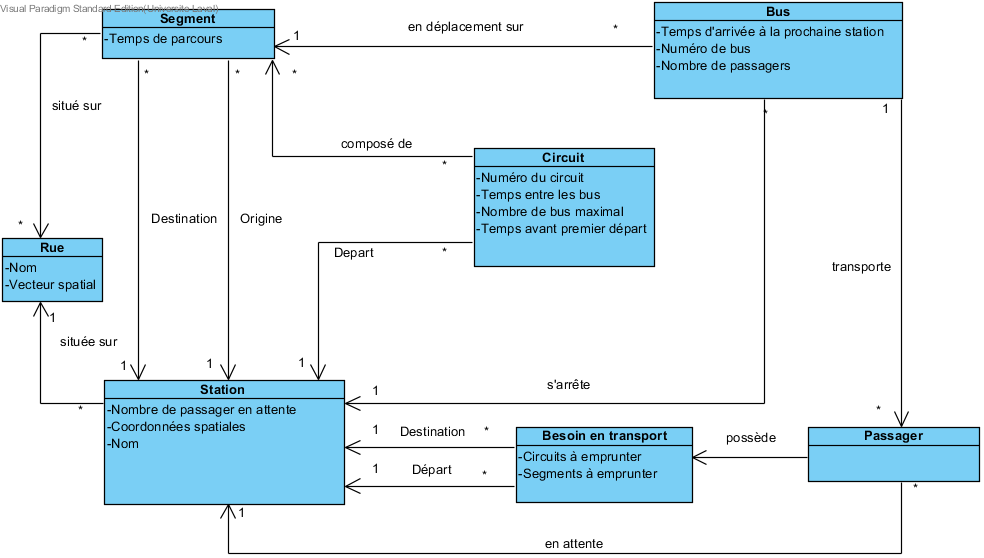
\includegraphics[scale=0.8]{fig/domainModel}
		\caption{Mod�le du domaine SimulatHEURE}
		\label{f:domainModel}
		\end{figure}



\end{document}          
